%%%%%%%%%%%%%%%%%%%%%%%%%%%%%%%%%%%%%%%%%%%%%%%%%%%%%%%%%%%%%%%%%%
%%%%%%%% CPSC 66 FALL 2021  REPORT %%%%%%%%%%%%%%%%%%%%%%%%
%%%%%%%% This template is modified from ICML 2014 %%%%%%%%%%%%%%%%
%%%%%%%%%%%%%%%%%%%%%%%%%%%%%%%%%%%%%%%%%%%%%%%%%%%%%%%%%%%%%%%%%%

\documentclass{article}

%include any external packages here.  This is similar to loading a
%library in python or C++

% use Times
\usepackage{times}
% For figures
\usepackage{graphicx}
\usepackage{lipsum}
% For citations
\usepackage{natbib}
\usepackage{subfigure}
% For algorithms and pseudocode
\usepackage{algorithm}
\usepackage{algorithmic}

%Adds hyperlinks to your citations automatically
\usepackage{hyperref}

%Package to help with formatting whitespace between list items
\usepackage{enumitem}

%Package to produce nicely formatted graphs
\usepackage{tikz}

%Correct weird RGB colors from tikz
\usepackage{xcolor}

\definecolor{pos}{RGB}{7,48,106}
\definecolor{neg}{RGB}{114,178,216}

% Packages hyperref and algorithmic misbehave sometimes.  We can fix
% this with the following command.
\newcommand{\theHalgorithm}{\arabic{algorithm}}

\usepackage[accepted]{icml2014}
\usepackage{array}
	
\usepackage{soul}
%\AtBeginEnvironment{figure}{\setlength{\intextsep}{3\ba%selineskip}}

% If your title is long (below), use this command to also provide
% short version.  This will go on the top of every page
\icmltitlerunning{Final Report}
\begin{document}

\twocolumn[ %use two column if you need a text to span across the whole page
\icmltitle{ CPSC 66 Final Report: \\ % \\ force a new line
Risk Factors Identification and Prediction of Long COVID }
%\bibliographystyle{abbrvnat}
\icmlauthor{Meiqing Jin}{mjin2@swarthmore.edu}
\icmlauthor{Elliot Kim}{ekim5@swarthmore.edu}
\icmlauthor{Xinwei Song}{xsong3@swarthmore.edu}

\vskip 0.3in
]

\begin{abstract}
% Why is long COVID worth studying -> Central goal
As of July 2021, long COVID, or post-COVID conditions, is officially considered a form of disability under the Americans with Disabilities Act (ADA) \citep{CDC}. Given the severe impacts long COVID incurs on patients who pulled through COVID-19 infection, we are interested in learning about the defining risk factors of long COVID, and consequently gain more insight in how to alleviate the suffering that long COVID causes.
% How machine learning comes into the project
Although it would be extremely difficult to identify risk factors of long COVID in a dataset by human eye, we can make use of machine learning models that either explicitly or implicitly exhibit feature importance.
% Results of the project (how our model performed, what we ultimately found)
After various experiments with different machine learning models, we ultimately chose the Random Forest Classifier as our optimal model. Our tuned model achieved a 0.723 accuracy and a precision of 0.815. We discovered that the presence of long COVID is strongly correlated with the severity of symptoms during COVID-19 infection.

\end{abstract}

\section{Introduction}
\label{introduction}
%It includes a definition of the problem you are solving, a description of why that problem is worth solving, and a high-level description of the solution(s) you apply to the problem. In addition, it motivates the work you are doing (i.e. why should a reader find your work important), and describes your contribution to the area (this may not be applicable to your project).

Since the advent of the COVID-19 pandemic, a wide range of symptoms and disease severity have been observed in patients. The scientific and medical communities have belabored themselves to answer the myriad questions surrounding a variety of COVID-19 manifestations. One phenomenon of COVID-19 that has been observed in a subpopulation of patients is the persistence of symptoms beyond otherwise complete recovery. “Long COVID,” as it is colloquially known, remains largely uncharacterized in terms of its causes and affected population.

Emerging studies on long COVID have investigated the mentioned persistence of symptoms and have found that they can last for weeks or months after a negative COVID test result \citep{DAVIS2021101019}. A study in Italy found that it is a rather prevalent phenomenon, as $35\%$ of outpatients and $87\%$ of inpatients for COVID-19 still experienced at least one symptom 60 days after discharge: this can be broken down into $32\%$ with one or two persistent symptoms and $55\%$ with three or more symptoms \citep{10.1001/jama.2020.12603}. A wide range of symptoms have been documented, of which patients can experience a diverse assortment. Among more than 50 long COVID-related symptoms studied, the five most common are fatigue ($58\%$ of long COVID patients), headache ($44\%$), attention disorder ($27\%$), hair loss ($25\%$), and shortness of breath ($24\%$) \citep{ssrn}. 

Key clinical challenges for long COVID include identifying patients particularly vulnerable to long COVID. Research on long COVID risk factors thus far has focused primarily on those related to symptoms and demographics. One early study found that women may be twice as likely as men to experience long COVID, and that the mean age of long COVID patients is four years greater than the mean age of non-long COVID patients \citep{Nabavim3489}. Another study with children found that comorbidities and having 5+ symptoms during acute COVID were correlated with a higher risk of long COVID \citep{Osmanov2101341}. Amid these few studies, even fewer examines potential socioeconomic and behavioral risk factors. Understanding these risk factors is critical to a holistic approach to medicine and public health, as they provide insight into the decision making space of patients as well as between patients and doctors, specifically environmental limitations and misinformation that may lead to suboptimal and misguided patient choices.

Uncovering risk factors in as complex and broad a problem as this is extremely impractical to do manually, but machine learning techniques allow exceedingly more facile and rapid analysis of a given dataset. Many machine learning models produce either explicit or implicit feature importances which are analogous to risk factors. 

Therefore, we decide to utilize machine learning to gain insight into the risk factors for long COVID. We are curious to see which particular algorithm(s) may yield the best performance for long COVID prediction, and then which risk factors our best model would identify in our dataset of COVID patients. To this end, we break down this project into two parts: first, build a classifier that accurately classifies whether a patient has long COVID. Then, based on the classifier, calculate the feature importances and identify the most defining risk factors for long COVID. Further analysis of the problem can be based on data acquired from the model.


\section{Methods}
\label{methods}
% A description of your approach to solving the task.  Provide algorithms, equations, descriptive figures, pseudocode, etc.

\subsection{Choosing the Classifiers}
In order to identify the best-performing model on the dataset, multiple classifiers are needed initially to provide grounds for comparison of their performance.
This section will provide a brief overview of the models used.

There are two main factors we take into consideration when choosing what classifiers we want to experiment on:
\begin{enumerate}[noitemsep]
    \item Since we have a set of binary labels \{$1:$ Patient has long COVID, $0:$ Patient does not have long COVID\}, we want to choose classifiers that are known to be more suitable for binary classification.
    \vspace{0.5em}
    \item All features in our dataset are categorical, i.e., values for each feature are discrete, with each value mapping to some category.
\end{enumerate}
Based on the two factors above, the following five classifiers are ultimately used: Logistic Regression \citep{10.2307/352104}, Naive Bayes \citep{10.2307/1403452}, Support Vector Machine \citep{Cortes1995}, Decision Tree \citep{Quinlan1986}, and Random Forest \citep{Breiman2001}.

\subsection{Building the Models}
All models used in this project are built using Python library scikit-learn \citep{scikit-learn}. 
For Logistic Regression, the Decision Tree, and the Random Forest, the baseline, default constructors are used.

For Naive Bayes, \texttt{ComplementNB()} , which is the Complement Naive Bayes classifier, is used. We chose this classifier instead of the Multinomial Naive Bayes classifier or the Gaussian Naive Bayes classifier because our dataset is severely imbalanced: among the subjects who were infected with COVID, over $60\%$ of them reported having some symptom(s) of long COVID, leaving only approximately $30\%$ of subjects without long COVID. The Complement Naive Bayes classifier is known to work better with imbalanced datasets.

For the Support Vector Machine, \texttt{SVC()}, which stands for the C-Support Vector Classification with a default 'rbf' kernel, is used. 

\subsection{Resampling the Data}

Resampling is a common method used to ``balance" imbalanced datasets. Class imbalance is exhibited when there is a significant difference between the amount of examples with each label. For example, in our dataset, we have over $60\%$ of patients with a positive label for long COVID, and only approximately half as many patients with a negative label. Imbalance of the dataset may severely impact the performance of a model.

There exists two main categories of resampling: upsampling and downsampling, or oversampling and undersampling. Upsampling generates more instances of the minority class, while downsampling cuts down on instances of the majority class. For the purposes of this project, we hope to at least preserve the original number of examples, since our dataset is not large. Therefore, we utilize upsampling, which generates more instances of ``patients" without long COVID in a way that's consistent with the original data. 

\begin{figure}[h]
\centering
\begin{tikzpicture}[x=1.2cm,y=1cm]
\tikzstyle{every node}=[font=\scriptsize]
%\filldraw[fill={rgb:red,114;green,178;blue,216}, draw=black]
    \filldraw[fill=neg, draw=white] (0,0) rectangle (0.8,0.5);
    \node[text width=0.01cm] at (0.08,-0.2) {negative};
    \filldraw[fill=pos, draw=white] (1,0) rectangle (1.8,1.5);
    \node[text width=0.01cm] at (1.1,-0.2) {positive};
    
    \draw [->,>=stealth] (2.3,.4) -- (3.5,.4);
    \node[text width=2.5cm] at (3.15,0.85) {Upsample examples with negative labels};
    
    \filldraw[fill=neg, draw=white] (4,0) rectangle (4.8,0.5);
    \node[text width=0.01cm] at (4.08,-0.2) {negative};
    \filldraw[fill=neg, draw=white] (4,0.5) rectangle (4.8,1);
    \filldraw[fill=neg, draw=white] (4,1) rectangle (4.8,1.5);
    \filldraw[fill=pos, draw=white] (5,0) rectangle (5.8,1.5);
    \node[text width=0.01cm] at (5.1,-0.2) {positive};
\end{tikzpicture}
\caption{Illustration of how upsampling works}
\label{fig:my_label}
\end{figure}

It is important to note that we only perform upsampling on the training set, since we want to avoid generating unreal examples to use for testing. In other words, while a new, more balanced training set is generated to train the models, the testing set preserves its class imbalance as a valid representation of the real-world population.


\subsection{The Gini Feature Importance for Random Forests}

An important goal of this project is to identify the most important risk factors that lead to long COVID. A machine learning model can assist this task by providing the feature weights, where each feature can be considered a risk factor that leads to what the label is measuring. Specifically, in Random Forests, the classifier that we ultimately chose, the Gini feature importance can be used as a general indicator of feature relevance to the label \citep{scikit-learn}.

Below is an algorithm to calculate the Gini Feature Importances for a Random Forest with binary class labels $\{0, 1\}$.

\begin{algorithm}
\caption{Calculate Gini Importance for Binary Labels}\label{alg:cap}
\begin{algorithmic}
    \FOR{each tree $T$}
      \FOR{each node $\tau$ in $T$}
      \STATE \textcolor{gray}{\COMMENT{Calculate Gini Impurity for binary class labels}}
      \STATE $i(\tau) = 1 - p_0^2 - p_1^2$ 
        \FOR{each available feature $\theta$ at $\tau$}
          \STATE \textcolor{gray}{\COMMENT{Calculate sample fractions for $\tau$'s children}}
          \STATE $p_l = \frac{n_l}{n}$, $p_r = \frac{n_r}{n}$ 
          \STATE \textcolor{gray}{\COMMENT{Record the decrease of Gini Impurity}}
          \STATE $\Delta i(\tau) = i(\tau) - p_l i(\tau) - p_r i(\tau)$ 
        \ENDFOR
      \ENDFOR
    \ENDFOR
    \STATE
    \FOR{each feature $\theta$}
      \STATE \textcolor{gray}{\COMMENT{Calculate Gini importance for each feature}}
      \STATE $I_G(\theta) = \sum_T \sum_\tau \Delta i_\theta (\tau, T)$
    \ENDFOR
\end{algorithmic}
\end{algorithm}

For each Decision Tree in the Random Forest, the Gini impurity (how much a feature decreases the impurity for the split) is measured for each feature by:
$$i(\tau) = 1 - p_0^2 - p_1^2$$

Then, the decrease of Gini impurity is calculated by:
$$\Delta i(\tau) = i(\tau) - p_l i(\tau) - p_r i(\tau)$$

If we record all Gini impurities for all nodes $\tau$ in all trees $T$, then we can finally calculate the Gini importance for feature $\theta$, $I_G(\theta)$, by the following equation:
$$I_G(\theta) = \sum_T \sum_\tau \Delta i_\theta (\tau, T)$$
(All equations above are cited from \citep{Menze2009}.)

In the context of this project, the attribute \texttt{feature\_importances\_} of the Random Forest classifier from scikit-learn is used. The feature importances are normalized such that they sum up to 1.

\subsection{Calculating Subgroup Percentages}
After acquiring the most important risk factors, we are curious to see in what direction each risk factor impacts the ultimate label. This can be done by examining the respective numbers of patients with positive and negative labels for each unique value of a risk factor.

If there exists $n$ unique values for a feature $\theta$, then for each unique value $v_i$ ($1 \leq i \leq n$), define $|v_i|$ to be the number of examples with value $v_i$ for feature $\theta$. Then, compute respective counts of examples with a positive label and with a negative label, which we define as $|v_{i,pos}|$ and $|v_{i,neg}|$. 

By comparing $|v_{i,pos}|$ and $|v_{i,neg}|$, we can gain insight on the label to which the value $v_i$ contributes. However, this could potentially be problematic since each value will likely have a different $|v_i|$. Thus, only analyzing the raw data may lead to biased results. To combat this, the data is normalized based on $|v_i|$, such that for each $v_i$, the percentage of examples with a positive label and that with a negative label sum up to 1. Mathematically, we calculate the positive and negative percentages as follows:
$$P_{pos} = \frac{|v_{i,pos}|}{|v_i|}, \hspace{0.1cm} P_{neg} = \frac{|v_{i,neg}|}{|v_i|}$$
In Fig. 2 below, $P_{pos}$ and $P_{neg}$ are plotted for patients who had access to internet, phone, tablet, computer, and audio/video during infection with COVID.
\begin{figure}[H]
    \center
    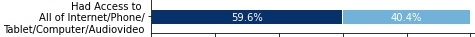
\includegraphics[width= \columnwidth]{pbv.jpeg}
    \caption{Illustration of percentages by value: examples grouped by positive and negative labels.}
    \vspace{-4mm}
\end{figure}
Due to the lack of a common term for these percentages, for clarity, we will refer to it as the PBV, which stands for ``Percentage By Value", for the remainder of this paper.


\section{Experiments and Results}
\label{results}
\subsection{Data Preprocessing}
The datasets used in this study are the Medicare Current Beneficiary Survey (MCBS) COVID-19 Community Supplements for Fall 2020 and Winter 2021 supplied by the Centers for Medicare and Medicaid Services (CMS). The two datasets are joined after ensuring that equivalent features were appropriately combined.

There are originally over 300 features ranging across patient demographics, barriers to care, preexisting health conditions, etc. To eliminate noise from the dataset and ensure better model performance, we performed feature selection by discarding redundant or distracting features (e.g., interview week), as well as feature extraction by transforming a group of features into one new feature (e.g., we combined access to Internet, access to computer, etc. into a single feature for digital access). Finally, after observing feature importances from our Random Forest classifier, we removed features with trivial weights, leaving a total of 51 features.

After filtering out participants who were not infected with COVID, the dataset consists of 615 long COVID patients and 286 non-long COVID patients. Evidently, the dataset is heavily imbalanced, resulting in poor precision scores for our models, as they tend to over-predict the number of patients with long COVID, as this would likely yield a decent accuracy. In order to address this, upsampling for non-long COVID patients was performed on the training set such that the number of long COVID and non-long COVID patients would be equal.

Since all our feature names and feature values are all in code names and integers respectively, we created dictionaries to map all these feature names and feature values into human readable terms. We apply dictionaries when plotting results containing feature names and values to provide human readable outcomes. 
\subsection{Experiments}

We first sought to identify the best performing algorithm out of the five chosen classifiers. To this end, we performed hold-out validation on each of the models. We further tuned each model on various sets of hyperparameters by running a five-fold validation test, where exhaustive Grid Search was performed on each fold to determine the optimal combination of hyperparameter values that would yield the highest tuning accuracy \citep{scikit-learn}. We computed the mean testing accuracy across the five folds for each tuned model, and ultimately determined that the Random Forest classifier was the best-performing model.

Proceeding with our Random Forest classifier, we analyzed the precision and recall scores using a confusion matrix. We discovered that our model was overly aggressive in predicting non-long COVID patients to be long COVID patients. To combat this, we analyzed validation curves of the model's five hyperparameters (number of estimations, max depth, max leaf nodes, max leaf nodes, max features and min samples leaf) to tune for precision. For example, the validation curve for the max depth hyperparameter (Fig. 3) reveals that a max depth greater than or equal to 5 optimizes the model's cross validation score. We thus adjusted the model's hyperparameter values such that precision is increased while high accuracy is maintained (more in 3.3 Results) to acquire our final model.

\begin{figure}[H]
    \center
    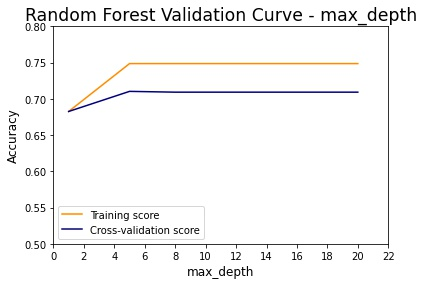
\includegraphics[width= \columnwidth]{Figure1.jpeg}
    \caption{Validation curves of hyperparameter ``max\_depth" of Random Forest. Cross validation score peaks after reaching 5.}
    \vspace{-5mm}
  \end{figure}

We want to further identify important risk factors that contributes to identifying cases of long COVID. After acquiring the Gini importance of each feature in our Random Forest model, we plotted the first ten features in a horizontal bar chart (Fig. 6). The most prominent features are ``Severity of COVID-19 Symptoms" and ``Sought medical care for COVID-19". 

Yet, knowing which features are the most important is not enough to fully understand the risk factors: we need to obtain specific feature values that contribute to identifying the labels. We first plotted the PBVs with the true labels of the first five most important features using the original dataset (first two features are shown in Fig. 7 and 8). We also plotted the PBVs with the predicted labels from our model of the first 5 most important features using our testing set (first two features are shown in Fig. 9 and 10). This way, we not only observe in what directions each value of the risk factors impacts label identification, but can also validate the performance of our model on the actual dataset. 

\subsection{Results}

\begin{table}[H]
\begin{tabular}{ l c c}
\hline
Model  & Initial Model & Mean Tuned  \\
Name & Accuracy & Testing Accuracy\\
\hline 
Logistic Regression & 0.660 & 0.686\\
Decision Tree & 0.626 & 0.624\\
Random Forest & 0.723 & 0.720\\
SVM &0.668 &0.693\\
Naive Bayes&0.618& 0.654\\
\hline
\end{tabular}
\caption{\label{tab:table-name} Initial accuracy and mean testing accuracy after tuning for all five models.}
\vspace{-0.5cm}
\end{table}


In order to select the model with the best performance, we acquired the accuracies of the baseline models as well as the average testing accuracies for the tuned models (see Table 1). The Random Forest classifier returned the highest initial accuracy of 0.723 and a tuned accuracy of 0.720.

\begin{figure}[H]
    \raggedright
    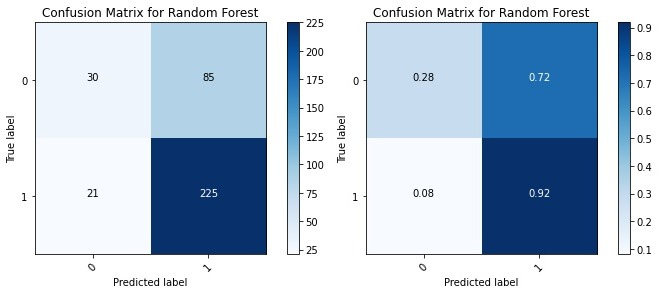
\includegraphics[width= \columnwidth]{Figure 2.jpg}
    \caption{Confusion Matrix vs Normalized Confusion Matrix for Random Forest before tuning.}
    \vspace{-0.5cm}
\end{figure}

According to the confusion matrix from the initial baseline Random Forest Model (Fig. 4), the model classified 226 true positive cases, 20 false negative cases, 35 true negative cases, and 80 false positive cases. The fact that there were more false positive cases than true negative cases revealed that our model was prone to classifying examples as positive. As our testing set was still highly imbalanced, this was even more evident in examining the normalized confusion matrix (Fig. 4), which yielded 0.92 true positives ratio, 0.08 false negatives ratio, 0.28 true negatives ratio, and 0.72 false positive ratio. 

\begin{figure}[H]
    \center
    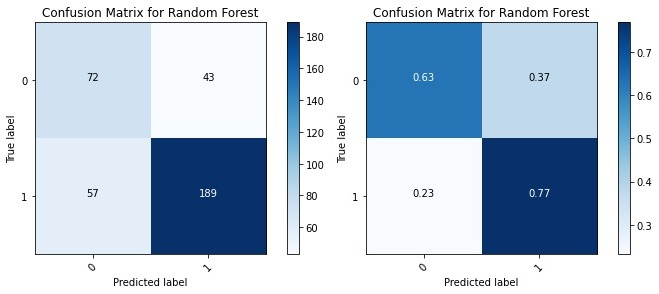
\includegraphics[width= \columnwidth]{Figure 3.jpg}
    \caption{Confusion Matrix vs Normalized Confusion Matrix for Random Forest after tuning.}
\end{figure}

After plotting the validation curves and adjusting the hyperparameters, our ultimate model has the hyperparameters: number of estimations = 75, max depth = 5, max leaf nodes = 15, max leaf nodes = 15, max features = $50\%$ and min samples leaf = 25. Performing a hold-out validation on this model yields accuracy = 0.723, precision = 0.815, recall = 0.768, and f1-score = 0.791. The confusion matrix for this final model exhibits 189 true positive cases, 57 false negative cases, 72 true negative cases, and 43 false positive cases. The normalized confusion matrix yielded 0.77 true positives ratio, 0.23 false negatives ratio, 0.83 true negatives ratio, and 0.37 false positive ratio. 

  \begin{figure}[H]
    \center
    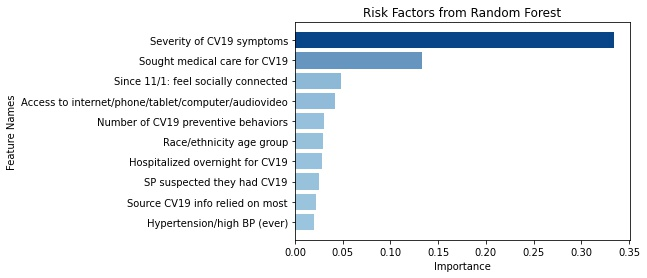
\includegraphics[width= \columnwidth]{Figure6.jpeg}
    \caption{Gini importances of the first ten features of Random Forest.}
  \end{figure}
  

The Gini importances of the the first ten features (Fig. 6) indicates the markedly greater importance of the first two features. While all the other features shown have importances of approximately 0.025 to 0.05, ``Severity of COVID-19 symptoms" scored an importance of 0.334 and ``Sought medical care for COVID-19" scored 0.133.

The PBVs of true labels of ``Severity of COVID-19 symptoms" (Fig. 7) indicates a direct relationship between the severity of COVID-19 symptoms and incidence of long COVID: $31\%$ of patients without symptoms, $55.9\%$ of patients with mild symptoms, $79.5\%$ of patients with moderate symptoms and $89.6\%$ of patients with severe symptoms experienced long COVID.

\begin{figure}[H]
    \center
    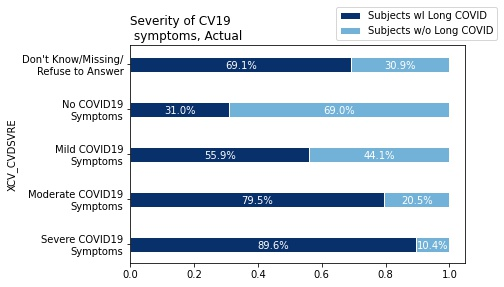
\includegraphics[width= \columnwidth]{Figure7.jpeg}
     \caption{True Label Percentages By Value for ``Severity of COVID-19 symptoms".}
     \vspace{-6mm}
  \end{figure}

  
The PBVs of true labels of "Sought medical care for COVID-19" (Fig. 8) shows that $79.5\%$ of patients who sought medical care for COVID-19, and $53.0\%$ of patients who did not seek medical care for COVID-19 have long COVID.

\begin{figure}[H]
    \centering
    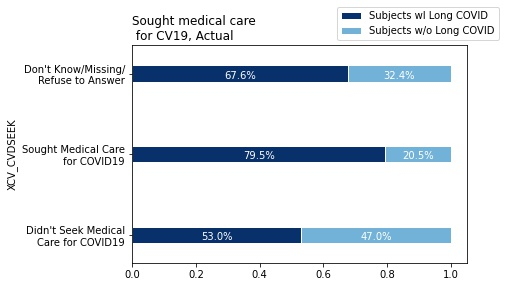
\includegraphics[width= \columnwidth]{Figure8.jpeg}
    \caption{True Label Percentages By Value for ``Sought medical care for COVID-19".}
    \vspace{-6mm}
  \end{figure}
 
The PBVs of predicted labels of ``Severity of COVID-19 symptoms" (Fig. 9) shows that our model classified $12.5\%$ of patients without symptoms, $27.9\%$ of patients with mild symptoms, $97.6\%$ of patients with moderate symptoms and $100\%$ of patients with severe symptoms as long COVID patients. 

\begin{figure}[H]
    \centering
    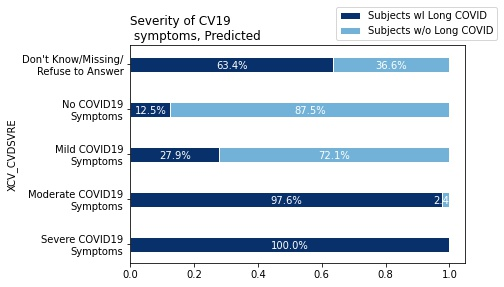
\includegraphics[width= \columnwidth]{Figure9.jpeg}
   \caption{Predicted Label Percentages By Value for ``Severity of COVID-19 symptoms".}
  \end{figure}
  

  \begin{figure}[H]
    \center
    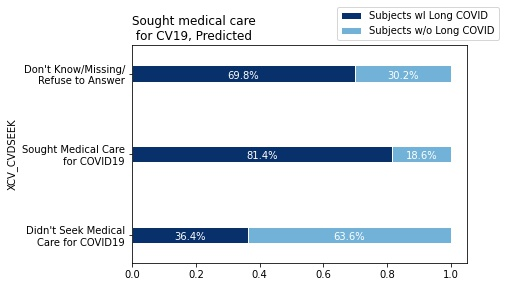
\includegraphics[width= \columnwidth]{Figure10.jpeg}
    \caption{Predicted Label Percentages By Value for ``Sought medical care for COVID-19".}
  \end{figure}

Upon comparing the figures, we can see that our model predicts in the same directions as the true labels, but tends to be slightly more extreme. 


\section{Discussion}
\label{discussion}
\subsection{Findings Explained}

Our findings show that the Random Forest classifier outperformed every other model both before and after tuning. It can correctly classify most examples with an accuracy of approximately $72\%$. This may be because Random Forest classifiers are particularly capable of learning diverse information as ensembles and have individual decision trees that are relatively shallow (or small), thus making them less prone to overfitting.

To identify the important risk factors, we plotted the Gini importances of the first ten features with highest feature importance. Out of these ten, the most prominent risk factors are ``Severity of COVID-19 symptoms" and ``Sought medical care for COVID-19". After examining the PBV graphs more closely, we found that as a general pattern, patients with more severe symptoms and patients who sought out medical care are more likely to have long COVID, which is reflected in our model predicting the same. This further supports our argument that the severity of COVID-19 symptoms has a positive correlation with getting long COVID.
\subsection{Clinical Implications} 

Our project discovered no notable correlations between long COVID and gender, and only discovered weak correlations between long COVID and the race/ethnicity/age group of the patient. These results differ with some existing literature on the risk factors of long COVID, where demographic info is highly correlated \citep{Nabavim3489} with long COVID. There are other literature that found comorbidities/pre-existing health conditions is one of the important risk factors for long COVID \citep{Osmanov2101341}. This is also not manifested in our results, with only ``Hypertension (ever)" as a weak top-10 risk factor. 

Instead, our findings that link severity of COVID-19 symptoms with long COVID reinforce the importance of existing and ongoing research dedicated to preventing and minimizing severe COVID-19.


\subsection{Social Implications}
Our model and results are primarily concerned with people who are or once were infected with COVID 19. This paper contributes to the growing literature on understanding and predicting long COVID. By identifying important risk factors, we hope to benefit people who already had COVID by providing them with more information to understand long COVID. And for people who are not infected with COVID-19, we want to point out our findings show that the risk of getting long COVID is high for patients with moderate to severe symptoms after infecting COVID. Although established treatment now exists for COVID-19, there is still no established cure or treatment for long COVID at the present \citep{apalongCOVID}. Also, our findings suggest that patients who only have mild COVID-19 symptoms can still get long COVID. This indicates a potential need for a shift in public health messaging to emphasize the risk of long COVID in patients who experience mild or even no COVID symptoms.

\section{Conclusions}
\label{conclusion}
To conclude, we built a model that predicts whether a patient will suffer from long COVID; our model exhibits moderate accuracy and precision. Given the feature importances extracted from this model, we discovered that the risk factors most strongly correlated with long COVID are the severity of COVID-19 symptoms exhibited and whether the patient sought medical care for COVID or not. This may potentially boil down to a single strong correlation with symptom severity of COVID-19, since patients seeking medical care may indicate them suffering from more severe symptoms (patients with less severe symptoms are more likely to stay at home and less likely to present to the hospital).

Then, after calculating the PBVs for the most important risk factors, we found that the more severe the symptoms during COVID infection are, the more likely a patient is going to suffer from long COVID. Interestingly, even COVID patients who exhibited no symptoms or mild symptoms during infection have a chance of over $30\%$ to have long COVID. We also found that patients who sought medical care are slightly more likely to have long COVID, which may be the outcome of different symptom severities, as mentioned above.

\subsection{Limitations}

\subsubsection{Limitations of Our Dataset}
We only have 901 examples (i.e., patients who were infected with COVID) in our original dataset to fit on a tailored set of 51 features. The size of our dataset limits us from reaching a higher of above $0.73$. Also, in our dataset, we are lacking specific information about patient demographic info (i.e., income, education, specific age), COVID symptoms, full descriptions on medical background and specific persistent symptoms. The lack of these information confines us from identifying more potentially important risk factors.  

\subsubsection{Limitations of Our Model}
Gini importance is used in our experiments to help identify important risk factors from our Random Forest Model. However, Gini importance potentially sabotages correlated features by only selecting one and ignoring others \citep{Strobl2007}. Thus, our feature importances could potentially ignore features that are correlated with the selected features.  


\subsection{Future Directions}

There are many future directions that can be taken to further investigate classifying long COVID and identifying important risk factors using machine learning. 

% What a more ideal dataset looks like

Since our dataset is relatively small and limited, in the future, it would be beneficial to have more data to train, tune and test on. A more ideal dataset should contain specific information about patient demographic info (i.e., income, education, specific age), COVID symptoms, fully descriptions on medical background and specific persistent symptoms to help understand the problem better. 

% How we could potentially improve our model
A direction in the future that can potentially improve our experiment is to explore other ways of calculating feature importance that do not potentially sabotage correlated features. 

Another direction that could be taken is to create a generative model with identifying probabilities of getting long COVID instead of classifying binary labels. For our problems, because we are trying to predict whether a once COVID patient has long COVID or not, a generative model is more flexible for it gives a probability instead of assigning binary outcomes.

% What our results suggest would be interesting future directions of research/ improvements
Based on the results of this project, one key future direction is to continue research on preventing and alleviating severe COVID, as symptom severity is what our results show to be most correlated with long COVID.
Also, these results indicate a potential need to reconsider the definition of ``full recovery" from COVID. At the present, if a COVID patient achieves a negative COVID test result, this is synonymous with recovery from COVID. However, as our results suggest, it may be worth considering the incorporation of the presence of symptoms into this definition, since COVID patients who test negative but still suffer persistent symptoms require continued medical attention.

\section*{Acknowledgments}


We would like to acknowledge MCBS for publishing their datasets for public use. We are also grateful to Ben Mitchell for his guidance and support throughout the whole process of this project. 


% In the unusual situation where you want a paper to appear in the
% references without citing it in the main text, use \nocite



\nocite{apalongCOVID}
\nocite{langley00}
\nocite{CDC}
\nocite{DAVIS2021101019}
\nocite{10.1001/jama.2020.12603}
\nocite{ssrn}
\nocite{Osmanov2101341}
\nocite{Nabavim3489}
\nocite{Strobl2007}
\nocite{scikit-learn}
\nocite{10.2307/352104} 
\nocite{10.2307/1403452} 
\nocite{Cortes1995}
\nocite{Quinlan1986}
\nocite{Breiman2001}
\nocite{Menze2009}
\bibliography{references}






\bibliographystyle{icml2014}

\end{document}


% This document was modified from the file originally made available by
% Pat Langley and Andrea Danyluk for ICML-2K. This version was
% created by Lise Getoor and Tobias Scheffer, it was slightly modified
% from the 2010 version by Thorsten Joachims & Johannes Fuernkranz,
% slightly modified from the 2009 version by Kiri Wagstaff and
% Sam Roweis's 2008 version, which is slightly modified from
% Prasad Tadepalli's 2007 version which is a lightly
% changed version of the previous year's version by Andrew Moore,
% which was in turn edited from those of Kristian Kersting and
% Codrina Lauth. Alex Smola contributed to the algorithmic style files.
